\section{Polarization ellipse derivation}
\label{sec:deriv_pol_ellipse}
Setting $kz-\omega t=\tau$ in the plane wave equations:
\begin{equation}
\begin{aligned}
    E_x(z, t) = E_{0x}\cos(\tau + \delta_x) \\
    E_y(z, t) = E_{0y}\cos(\tau + \delta_y).
\end{aligned}
\end{equation}
In order to eliminate $\tau$ we write the previous equations as:
\begin{equation}
\begin{aligned}
    \frac{E_x}{E_{0x}} = \cos(\tau)\cos(\delta_x) - \sin(\tau)\sin(\delta_x)\\
    \frac{E_y}{E_{0y}} = \cos(\tau)\cos(\delta_y) - \sin(\tau)\sin(\delta_y).
\end{aligned}
\end{equation}
Multiplying by $\cos(\delta_{x,y})$, $\sin(\delta_{x,y})$ subtracting and using trig. angle difference formulas we get:
\begin{equation}
\begin{aligned}
    \frac{E_x}{E_{0x}}\sin(\delta_y) - \frac{E_y}{E_{0y}}\sin(\delta_x) = \cos(\tau)\sin(\delta_y-\delta_x)\\
    \frac{E_x}{E_{0x}}\cos(\delta_y) - \frac{E_y}{E_{0y}}\cos(\delta_x) = \sin(\tau)\sin(\delta_y-\delta_x).
\end{aligned}
\end{equation}
Squaring and adding these two equations gives:
\begin{equation}
    \left(\frac{E_x}{E_{0x}}\right)^2+\left(\frac{E_y}{E_{0y}}\right)^2-2\frac{E_x E_y}{E_{0x} E_{0y}}\cos \delta =\sin^2 \delta,
\end{equation}
with $\delta=\delta_y-\delta_x$.

%\section{Index ellipsoid procedure}
%\label{sec:index_ellipse_proof}
% TODO remove? yes. (done)
% laser book

\section{Effective permittivity inequality}
\label{sec:bf_proof}
We want to show that $\epsilon_{s}<\epsilon_{p}$, where $\epsilon_{s}$ and $\epsilon_{p}$ are given in equation \ref{eq:rytov_2nd_order_final}. We assume that $1\leq\epsilon\leq4$ and that the ratio $r=\frac{d}{\lambda}$ is less than $0.6$ which is reasonable considering the condition stated in equation \ref{eq:rytov_cond1}. In order to slightly simplify the equations we can measure lengths in units of $d$ this means that $a+b=1$ or setting $a=f$ we end up with the following inequality we want to show:
\begin{equation}
    \label{eq:inequality_proof}
    0<1+\frac{\tilde{\epsilon}_{p}-\tilde{\epsilon}_{s}}{f^2(1-f)^2(\epsilon-1)^2c}-\frac{\tilde{\epsilon}_{p}\tilde{\epsilon}_{s}^3}{\epsilon^2},\quad c=\frac{1}{3}r^2\pi^2.
\end{equation}

Although, showing that this is true is fairly lengthy, we therefore only briefly describe the underlying idea. Since $\epsilon$ is bounded by $1$ and $4$ we can show that the right side of equation \ref{eq:inequality_proof}, which is a function of $\epsilon$ and $f$, is decreasing or increasing on some subset of the interval or the full interval if possible. If the right side is found to be increasing(decreasing) then we can simply show that the inequality is true at the lower(upper) bound of the interval. To show that the function is increasing(decreasing) we calculate the derivative with right to $\epsilon$ and show that it is strictly positive(negative), this gives us a new reduced inequality. Since equation \ref{eq:inequality_proof} is a polynomial the process will eventually terminate and we obtain simple inequalities for different subsections of the interval $[1,4]$. Doing this we were able to show that the inequality given in \ref{eq:inequality_proof} is true on the given interval and for all $f$ in $[0,1]$.

% Jan measurement setup (done)
\section{Transmission minimum of diattenuating linear retarder} 
\label{sec:transmission_min}
The setup consists of a linear horizontal polarizer $\hat{T}_{DL}(\psi=0, p_1=1, 0)$, linear diattenuating retarder (waveplate) $\hat{T}_{RDL}(\psi, \Delta, p_1, p_2)$ and another linear horizontal polarizer $\hat{T}_{DL}(\psi=0, p_1=1, 0)$ in the given order. The input is a normalized horizontal linear state $\bm{\mathcal{E}}_{\SI{0}{\degree}}$. The intensity of the output is then simply $I_o=T_{1,1}(T_{1,1})^*$, requiring $I_o\overset{!}{=}0$ we get the following:
\begin{equation}
    0=(p_1c_\psi^2e^{i\Delta/2}+p_2s_\psi^2e^{-i\Delta/2})(p_1c_\psi^2e^{-i\Delta/2}+p_2s_\psi^2e^{i\Delta/2}).
\end{equation}
Simplifying:
\begin{equation}
    \label{eq:trans_min_app}
    -2p_1p_2c_\Delta = p_1^2\left(\frac{c_\psi}{s_\psi}\right)^2 + p_2^2\left(\frac{s_\psi}{c_\psi}\right)^2
\end{equation}
The image of LHS is the interval $\left[-2p_1p_2, 2p_1p_2\right]$ while the image of the RHS is $\left[2p_1p_2, \infty\right)$. This means that equation \ref{eq:trans_min_app} only has a solution when
\begin{equation}
    c_\Delta=-1
\end{equation}
and
\begin{equation}
    2p_1p_2 = p_1^2\left(\frac{c_\psi}{s_\psi}\right)^2 + p_2^2\left(\frac{s_\psi}{c_\psi}\right)^2.
\end{equation}
From the first equation it follows that $\Delta=\pi$, $(\Delta \in [0,\pi])$ and the second equation is solved by:
\begin{equation}
    \label{eq:psi_min}
    \psi = \arctan \sqrt{\frac{p_2}{p_1}},
\end{equation}
that is, the intensity is zero for this $\psi=\psi_{min}$ given by equation \ref{eq:psi_min}.

\section{Basin-hopping algorithm}
\label{sec:basin_hopping_algo}

Basin-hopping is a stochastic algorithm which is used in global optimization problems and was first developed to solve problems in chemical physics \cite{Wales1997}. It is well suited for the optimization problems presented in this work, since it is an effective algorithm in the case of high dimensional smooth nonlinear loss functions $L(x)$ with multiple optima separated by large barriers \cite{Olson2012, Wu2020}. The algorithm mainly consists of cycling through three steps until some stop criterion is fulfilled. First a perturbation of a candidate solution is performed, then a local search is applied to the perturbed solution and then finally the coordinates are accepted or rejected based on the minimized function value. The associated pseudocode is shown in algorithm \ref{algo_bh}. 

\begin{algorithm}[H]
    \SetAlgoLined
    \SetKwFunction{LOCALSEARCH}{LOCALSEARCH}\SetKwFunction{STOP}{STOP}\SetKwFunction{PERTURB}{PERTURB}
    \SetKwFunction{METROPOLIS}{METROPOLIS}
    \SetKw{KwOr}{or}
    \SetKwData{NS}{not satisfied} \SetKwData{RP}{random initial point in variable space}
    
    $i \leftarrow 0$\;
    $x_i \leftarrow $ \RP\;
    $y_i \leftarrow $ \LOCALSEARCH{$x_i$}\;
    \While{\STOP \NS}{
        $x_{i+1} \leftarrow $ \PERTURB{$y_i$}\;
        $y_{i+1} \leftarrow $ \LOCALSEARCH{$x_i$}\;
        \If{$L(y_{i+1})<L(y_i)$ \KwOr{} \METROPOLIS{$y_{i+1}, y_i$}}{
            $i \leftarrow i+1$\;
        }
    }


\caption{Basin-hopping pseudocode}\label{algo_bh}
\end{algorithm}

Since we can not determine if the global minimum has actually been found for stochastic global optimization problems the \texttt{STOP} criterion is simply a number of iterations. The result is then the lowest minimum found. The additional acceptance criterion \texttt{METROPOLIS} is true with a probability $P(y_{i+1}, y_i)$ given by the following:
\begin{equation}
    P(y_{i+1}, y_i) = \exp\left(\frac{L(y_{i})-L(y_{i+1})}{T} \right),
\end{equation}
where $T$ is known as the temperature and is a user defined parameter which should be set similar to the average function value difference between local minima \cite{2020SciPy-NMeth}. The \texttt{LOCALSEARCH} step is in our case perfomed by the L-BFGS-B local optimization routine which is a quasi-Newton algorithm and allows the specification of bounds \cite{Byrd1995}. \texttt{PERTURB} is responsible for taking a step in variable space with a stepsize $\tau$ which is another user defined parameter. $\tau$ is an important parameter in Basin-hopping and depends on the optimization problem. The step is chosen uniformly in the region from $x-\tau$ to $x+\tau$, in each dimension. The Python implementation of the algorithm as we use it automatically adjusts the stepsize. Nevertheless, to achieve faster convergence the initial value should be similar to the average separation between local minima in variable space \cite{ScipyBH}. 

% TODO rewrite caption below (done)
\begin{figure}[h]
    \centering
    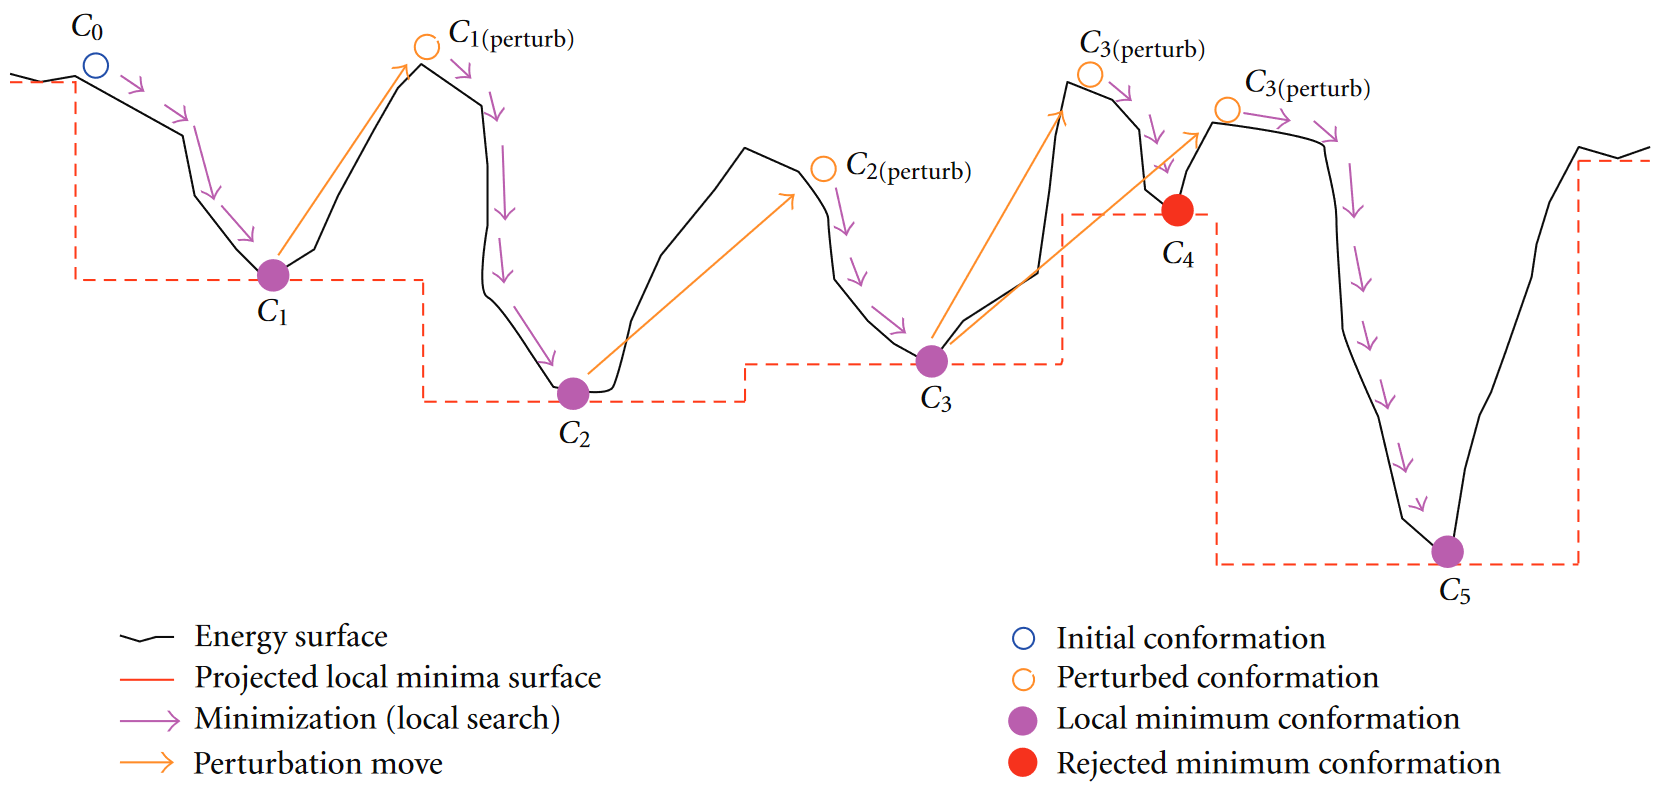
\includegraphics[scale=0.3]{images/appendix/bh.png}
    \caption{The Basin-hopping algorithm can be visualized as a transformation of the loss function (black line) into single steps(dotted line). 
    The local optimization routine is illustrated by purple arrows while the random perturbation is represented by yellow arrows. At $C_3$ the perturbation move fails the Metropolis acceptance criterion since the barrier is too high, a new perturbation move to a more favorable position is therefore made. Source: \cite{Olson2012}.}
    \label{fig:Basin-hopping}
\end{figure}

\section{Quartz Sellmeier approximation}
\label{sec:sellmeier}
In \cite{DGrischkowsky1990} the optical parameters along the fast and slow direction of crystalline quartz in the frequency range \SIrange{0.2}{2.0}{\tera\hertz} were published. The result was obtained through a measurement similar to the THz-TDS measurements performed in this work. In order to obtain an interpolation of the refractive indices with a sufficiently high accuracy from the publication we fitted the 3rd order Sellmeier relation which is given by the following expression:

\begin{equation}
    \label{eq:sellmeier}
    n^2(\lambda) - 1 = \frac{A_1\lambda^2}{\lambda^2-B_1}+\frac{A_2\lambda^2}{\lambda^2-B_2}+\frac{A_3\lambda^2}{\lambda^2-B_3},
\end{equation}

where the $A_j$, $B_j$ are fit parameters determined empirically and $\lambda$ is the wavelength in micrometres \cite{Sellmeier1872}. It is worth noting that the same method is used in \cite{Vilas2013} to obtain the wavelength dependency of the refractive indices along the two axes of \ce{MgF2} which are also used for the design development of an AWP. Furthermore, we fitted a polynomial to interpolate the absorption coefficients. The data points obtained from \cite{DGrischkowsky1990} as well as the corresponding fits for the refractive indices and absorption coefficients are shown in figures \ref{fig:ri_quartz} and \ref{fig:abs_quartz} respectively. The fitted Sellemeier coefficients are shown in table \ref{tab:sellmeier_parameters_table}. Since the refractive indices and absorption coefficients of the fast and slow axes are fairly smooth the fits are quite close to the data points. We use these fitted values for the calculations based on the optical parameters of crystalline quartz to reproduce the TAQ design.

\begin{figure}[H]
    \centering
    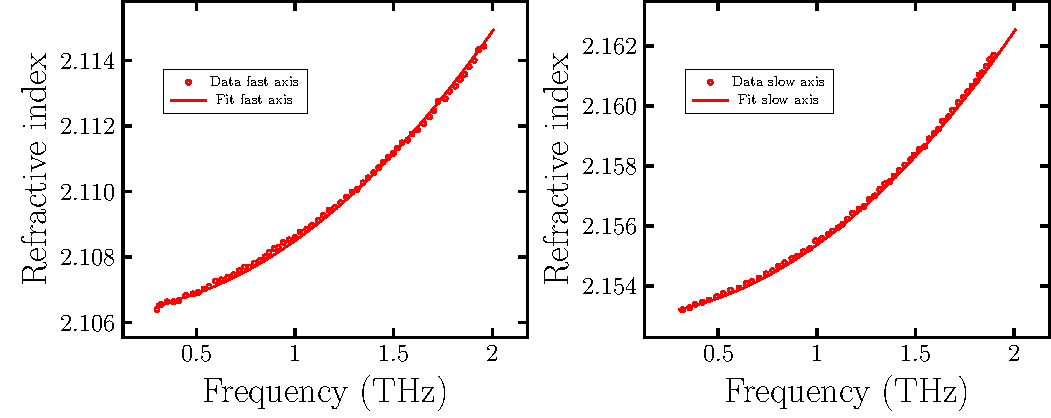
\includegraphics[scale=0.7]{images/appendix/plots/quartz_fits/ri_quartz.pdf}
    \caption{Refractive index of crystalline quartz along the fast (left subfigure) and slow (right subfigure) direction. Data points are obtained from \cite{DGrischkowsky1990} and subsequently used to fit the parameters of equation \ref{eq:sellmeier}.}
    \label{fig:ri_quartz}
\end{figure}

\begin{figure}[H]
    \centering
    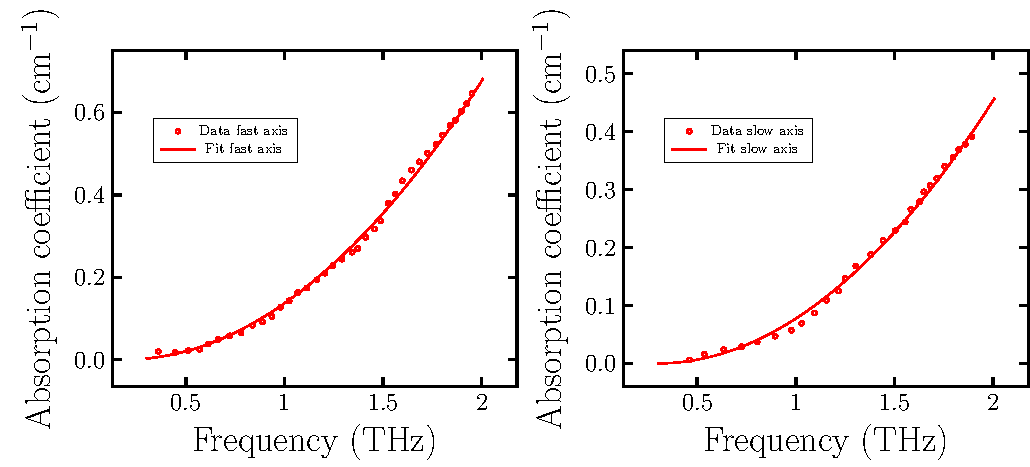
\includegraphics[scale=0.7]{images/appendix/plots/quartz_fits/abs_quartz.pdf}
    \caption{Absorption coefficient of crystalline quartz along the fast (left subfigure) and slow (right subfigure) direction. Data points are obtained from \cite{DGrischkowsky1990} which are used to determine the coefficients of a polynomial fit.}
    \label{fig:abs_quartz}
\end{figure}

\begin{table}[H]
    \centering
    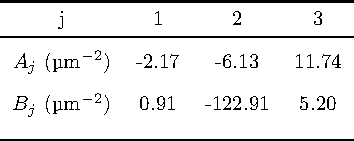
\includegraphics[scale=0.9]{images/appendix/sellmeier_parameters_table.pdf}
    \caption{Sellmeier parameters of crystalline quartz obtained from the fit of equation \ref{eq:sellmeier} to the measurement result published in \cite{DGrischkowsky1990}.}
    \label{tab:sellmeier_parameters_table}
\end{table}

\section{Stratified structure CST simulation}
\label{sec:CST simulation}
In order to obtain the form birefringence of a single stratified structure numerically we performed a unit cell simulation in the frequency domain of the structure shown in figure \ref{fig:CST_model}. For this type of simulation the unit cell is assumed to be repeating itself infinitely in the x- and y-direction according to the coordinate system shown in the figure, this saves a lot of memory and computing time and is nevertheless a good model of the real structure. The lower part of the unit cell (light blue) represents the material which in this case is modeled using the measured optical parameters of HIPS and the upper part represents the air gap ($n=1$, dark blue). To model the grating the height (y-direction) of the HIPS and air layer is therefore $a=\SI{735}{\micro \meter}$ and $b=\SI{393}{\micro \meter}$ respectively. The thickness of the grating $d$ is measured by the z-coordinate and is variable. 

\begin{figure}[H]
    \centering
    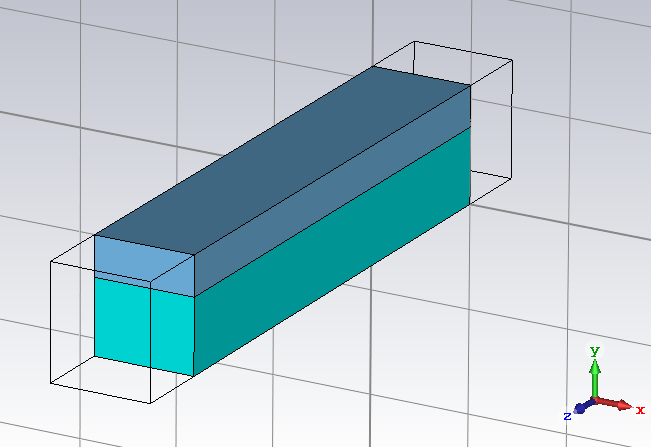
\includegraphics[scale=0.3]{images/appendix/CST.PNG}
    \caption{Unit cell of the structure representing a stratified medium with $a=\SI{735}{\micro \meter}$ and $b=\SI{393}{\micro \meter}$.}
    \label{fig:CST_model}
\end{figure}

This means that if we assume that the structure is birefringent and the incoming radiation is linearly polarized at \SI{45}{\degree} then for some frequency we expect that the magnitude of the field perpendicular to the input given by $|S_{21}|$ attains a minimum. In other words the effect of a half waveplate which means that equation \ref{eq:thickness_half_waveplate} is satisfied and we can rewrite it as follows:
\begin{equation}
    \frac{2d}{\lambda_0}=|n_o-n_e|=\Delta n,
\end{equation}
where we assume that the order is zero. Therefore, varying $d$ in small steps and determining $\lambda_0=\argmin|S_{21}(\lambda)|$ we can obtain the birefringence at $\lambda_0$. Figure \ref{fig:bf_sim} shows $|S_{21}|$ as a function of the frequency for the integer values of $d$.

\begin{figure}[H]
    \centering
    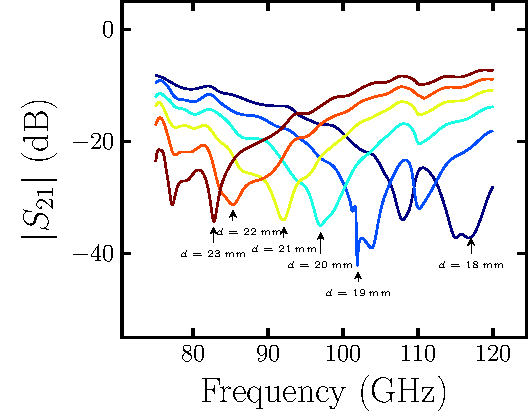
\includegraphics[scale=1]{images/appendix/plots/cst_sim/bf_sim.pdf}
    \caption{$|S_{21}|$ as a function of frequency obtained through the simulation of the unit cell shown in figure \ref{fig:CST_model} for different thicknesses of the structure.}
    \label{fig:bf_sim}
\end{figure}

\chapter{Characterization of ceramic material samples}
%\setcounter{page}{1} % remove in thesis version
\label{sec:ceramic_characterization}
\section{Description}
The 10 different material samples shown in figure \ref{fig:ceramic_samples} were characterized regarding their birefringence. To that extend each sample was placed in the focus of the two leftmost off axis parabolic mirrors as shown in figure \ref{fig:THz-TDS-HHI} (a). The sample holder is shown in figure \ref{fig:THz-TDS-HHI} (b) which enables a \SI{360}{\degree} manual rotation of the sample in the direction of the red arrow. The blue arrow in (a) and (b) indicates the polarization plane of the incident THz pulse. Each sample was placed in the holder so that the printing direction was approximately aligned with the \SI{0}{\degree} and \SI{180}{\degree} direction. Some samples were without a flat side but instead had an arrow drawn on them. In those cases we aligned the arrow so that it was parallel to the polarization of the THz radiation. At \SI{0}{\degree} the polarization plane and the printing direction of the 10 samples therefore align and at \SI{90}{\degree} they are orthogonal as shown in (b). 

\begin{figure}
    \centering
    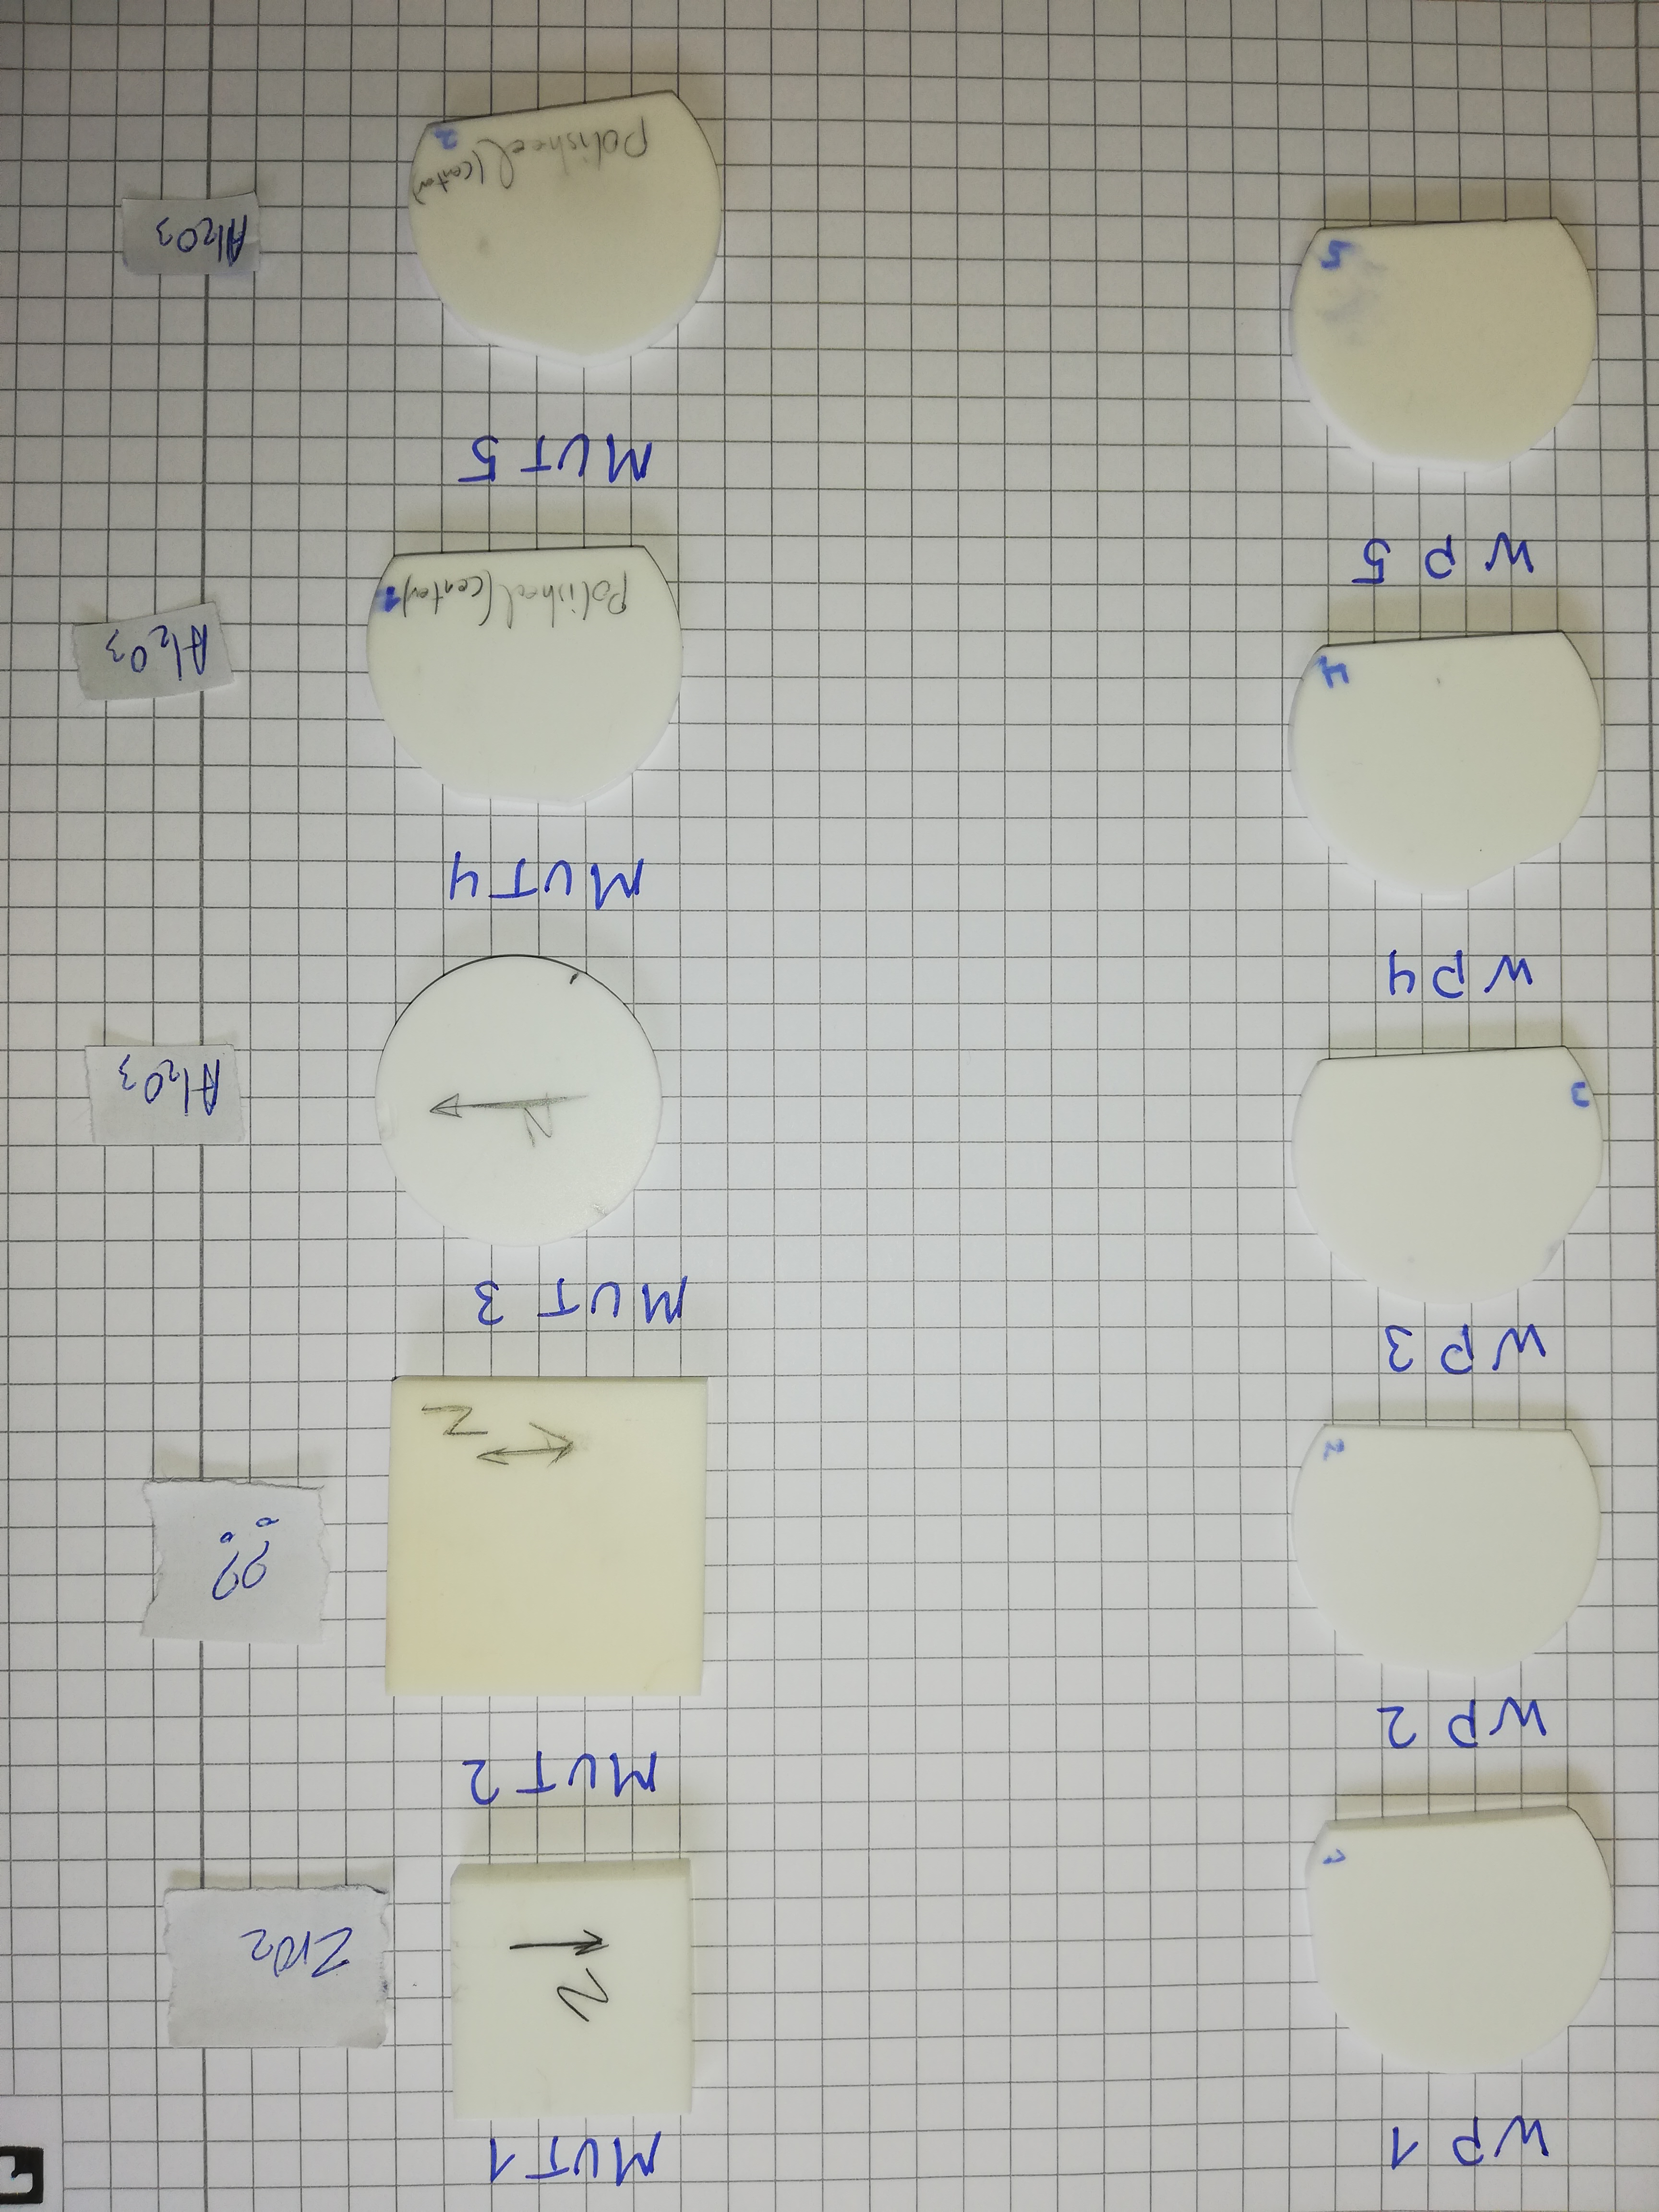
\includegraphics[scale=0.1,angle=180,origin=c]{images/appendix/ceramic_samples.jpg}
    \caption{Photo of the 10 characterized samples}
    \label{fig:ceramic_samples}
\end{figure}

\begin{figure}[H]
    \centering
    \subcaptionbox{\label{fig:setup_1}}
        {\hspace*{-2em}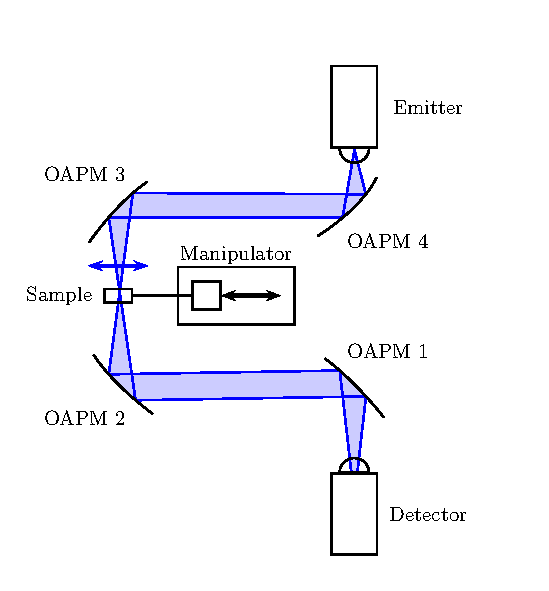
\includegraphics[width=0.45\linewidth]{images/appendix/Setup-THz-TDS-HHI.pdf}}
    \qquad
    \subcaptionbox{\label{fig:setup_2}}
        {\hspace*{-2em}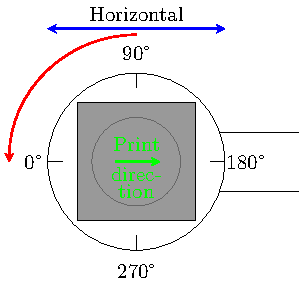
\includegraphics[width=0.45\linewidth]{images/appendix/sample_mount.pdf}}
    
    \caption{Subfigure (a): Main components of the measurement setup which consists of four off axis parabolic mirros, the sample mounted on a translation stage(manipulator) as well as the emitter and detector. Subfigure (b): Sample placed on a rotational mount. The blue arrow indicates the horizontal direction which is also the polarization plane of the incident radiation. The red arrow indicates the turn direction and the green arrow the direction in which the sample was printed.}
    \label{fig:THz-TDS-HHI}
\end{figure}

Each measurement was taken with a relative humidity of less than \SI{1}{\percent} and a mechanical stage was used to move the sample out of the beam path for a reference measurement. Due to the relative long nitrogen purge time and the manual sample rotator we measured each sample at three angles; \SI{0}{\degree}, \SI{90}{\degree} and \SI{180}{\degree}.
Table \ref{tab:ceramic_samples_table} lists the 10 samples, their respective handles which is used later and their respective measured thickness. The thickness was determined approximately at the center of each sample using a micrometer screw gauge. This thickness was then used for extraction of the refractive index for all three sample orientations. 

\begin{table}[h]
    \centering
    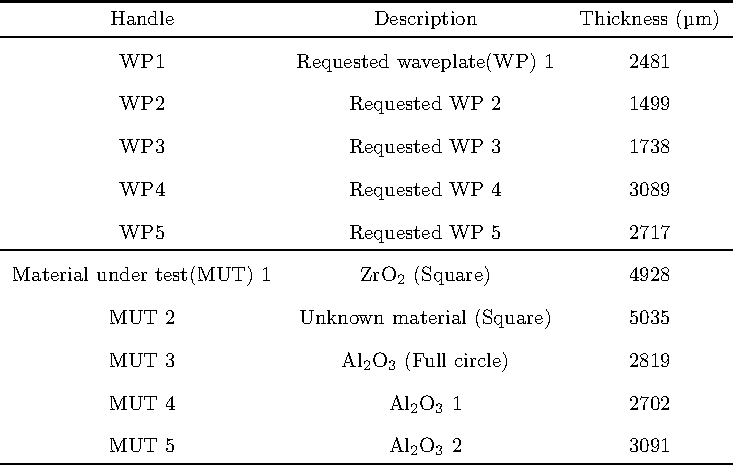
\includegraphics[scale=1.0]{images/appendix/ceramic_samples_table.pdf}
    \caption{The 10 characterized samples. The first five are the samples requested for the achromatic waveplate while the five in the lower half are the additionally characterized samples. The thickness is measured once at the center of the each sample using a micrometer.}
    \label{tab:ceramic_samples_table}
\end{table}

\newpage

\section{Results}
The data collected from the measurements was evaluated using the commercial software Teralyzer. We used the same thickness for all three angles for a given sample to be able to compare the refractive index at the three different rotational angles. The thicknesses used for the evaluation of each sample is given in \ref{tab:ceramic_samples_table}. 
It is possible to leave the thickness as a free parameter which can then be fitted and thereby slightly adjusted for each measurement to remove or reduce the oscillations seen in for example WP2 at \SI{0}{\degree}. Although, this introduces a slight frequency independent offset in the refractive index which depends on the fitted thickness and thereby changes the measured birefringence. We therefore chose to use one thickness for all three angles. 

Figure \ref{fig:ceramic_WPs} shows the evaluated refractive index at the three angles for the requested waveplates 1-5 and figure \ref{fig:ceramic_MUTs} shows the results of the evaluation for the additional five samples. The strong attenuation of MUT1 limited the usable frequency range to \SI{0.8}{\tera \hertz}. 

\begin{figure}[H]
\centering
\subcaptionbox{\label{fig:ceramic_WP1}}
    {\hspace*{-2em}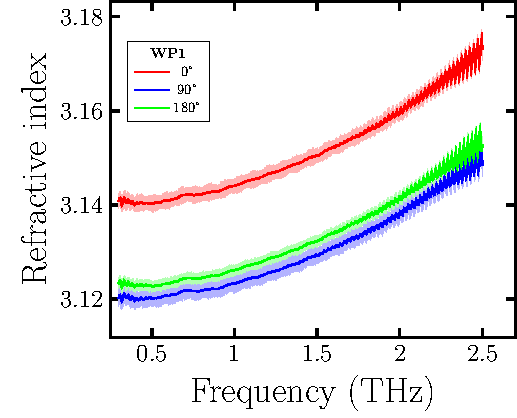
\includegraphics[width=0.45\linewidth]{images/appendix/plots/real/WP1.pdf}}
\qquad
\subcaptionbox{\label{fig:ceramic_WP2}}
    {\hspace*{-2em}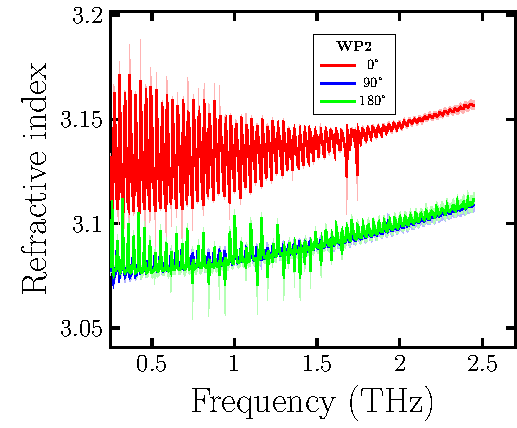
\includegraphics[width=0.45\linewidth]{images/appendix/plots/real/WP2.pdf}}
\subcaptionbox{\label{fig:ceramic_WP3}}
    {\hspace*{-2em}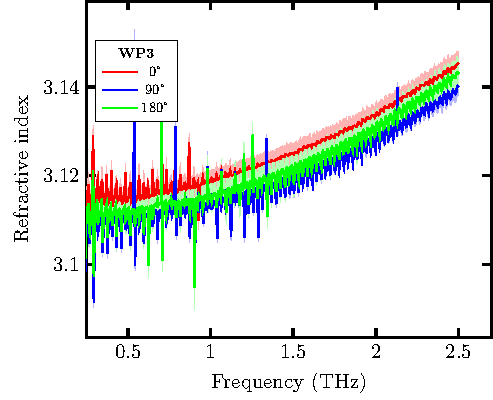
\includegraphics[width=0.45\linewidth]{images/appendix/plots/real/WP3.pdf}}
\qquad
\subcaptionbox{\label{fig:ceramic_WP4}}
    {\hspace*{-2em}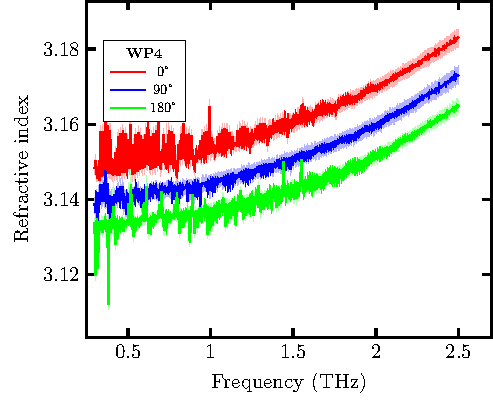
\includegraphics[width=0.45\linewidth]{images/appendix/plots/real/WP4.pdf}}
\subcaptionbox{\label{fig:ceramic_WP5}}
    {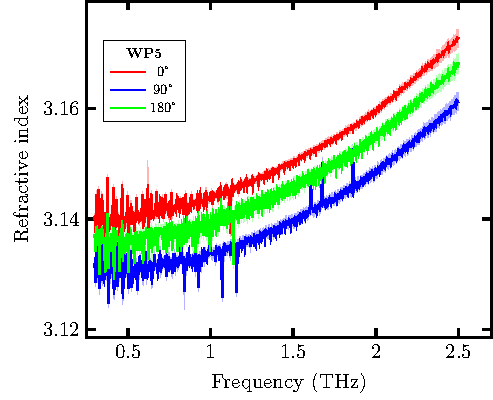
\includegraphics[width=0.45\linewidth]{images/appendix/plots/real/WP5.pdf}}
\caption{Evaluated refractive index for the five requested waveplates at three different rotational angles.}
\label{fig:ceramic_WPs}
\end{figure}

\begin{figure}[H]
\centering
\subcaptionbox{\label{fig:ceramic_MUT1}}
    {\hspace*{-2em}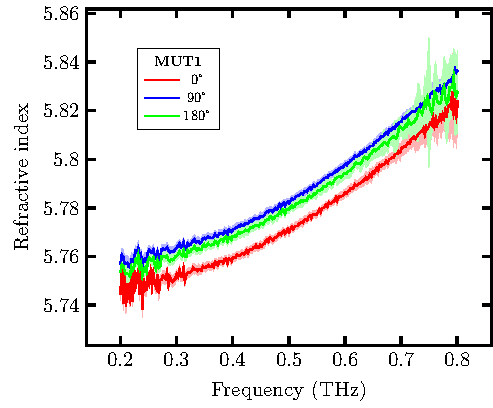
\includegraphics[width=0.45\linewidth]{images/appendix/plots/real/MUT1.pdf}}
\qquad
\subcaptionbox{\label{fig:ceramic_MUT2}}
    {\hspace*{-2em}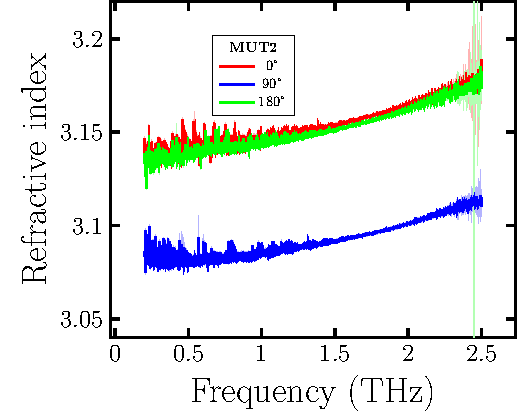
\includegraphics[width=0.45\linewidth]{images/appendix/plots/real/MUT2.pdf}}
\subcaptionbox{\label{fig:ceramic_MUT3}}
    {\hspace*{-2em}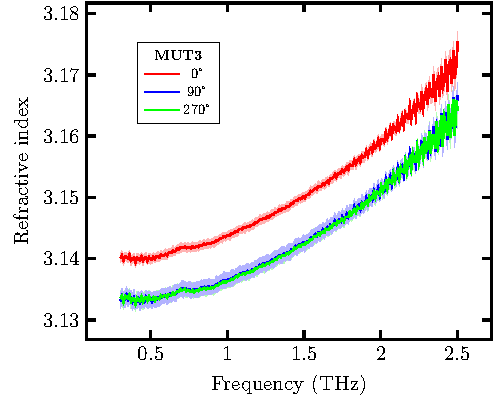
\includegraphics[width=0.45\linewidth]{images/appendix/plots/real/MUT3.pdf}}
\qquad
\subcaptionbox{\label{fig:ceramic_MUT4}}
    {\hspace*{-2em}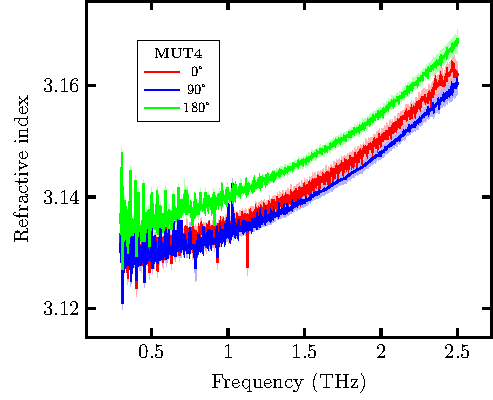
\includegraphics[width=0.45\linewidth]{images/appendix/plots/real/MUT4.pdf}}
\subcaptionbox{\label{fig:ceramic_MUT5}}
    {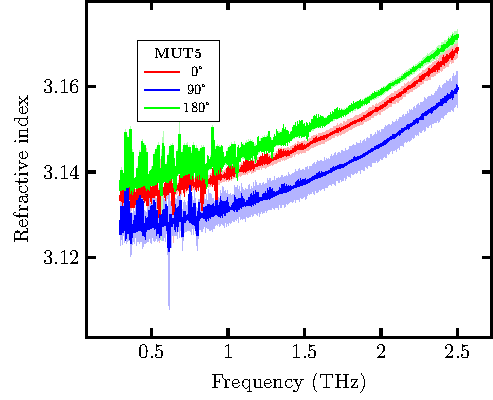
\includegraphics[width=0.45\linewidth]{images/appendix/plots/real/MUT5.pdf}}
\caption{Evaluated refractive index for the five additional samples at three different rotational angles.}
\label{fig:ceramic_MUTs}
\end{figure}

\begin{figure}[H]
\centering
\subcaptionbox{\label{fig:ceramic_WP1_abs}}
    {\hspace*{-2em}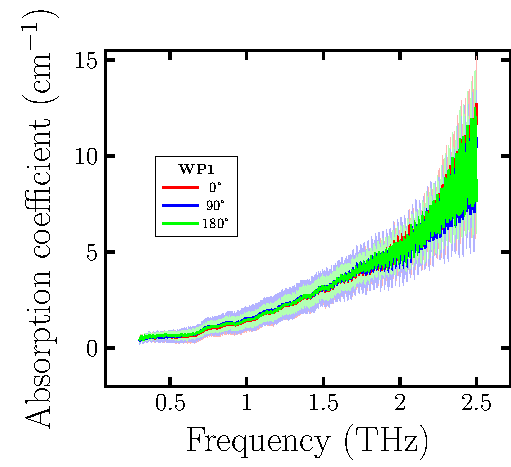
\includegraphics[width=0.45\linewidth]{images/appendix/plots/real_abs/WP1.pdf}}
\qquad
\subcaptionbox{\label{fig:ceramic_WP2_abs}}
    {\hspace*{-2em}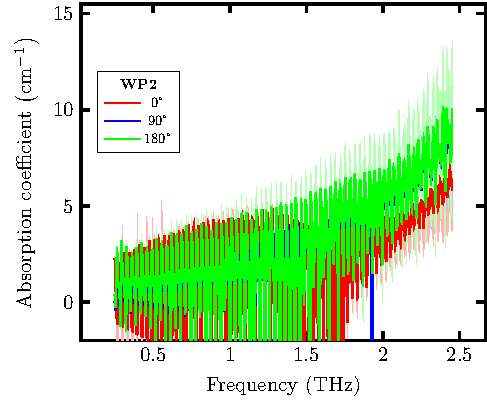
\includegraphics[width=0.45\linewidth]{images/appendix/plots/real_abs/WP2.pdf}}
\subcaptionbox{\label{fig:ceramic_WP3_abs}}
    {\hspace*{-2em}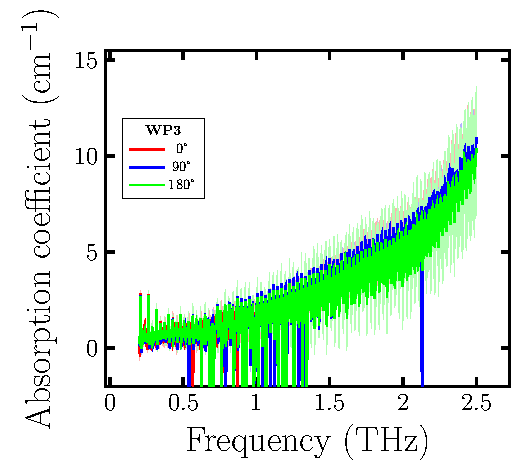
\includegraphics[width=0.45\linewidth]{images/appendix/plots/real_abs/WP3.pdf}}
\qquad
\subcaptionbox{\label{fig:ceramic_WP4_abs}}
    {\hspace*{-2em}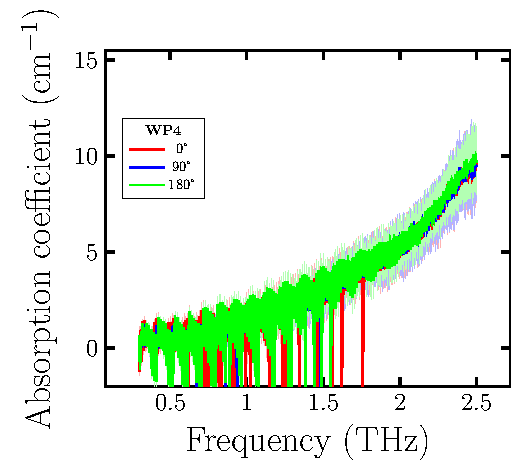
\includegraphics[width=0.45\linewidth]{images/appendix/plots/real_abs/WP4.pdf}}
\subcaptionbox{\label{fig:ceramic_WP5_abs}}
    {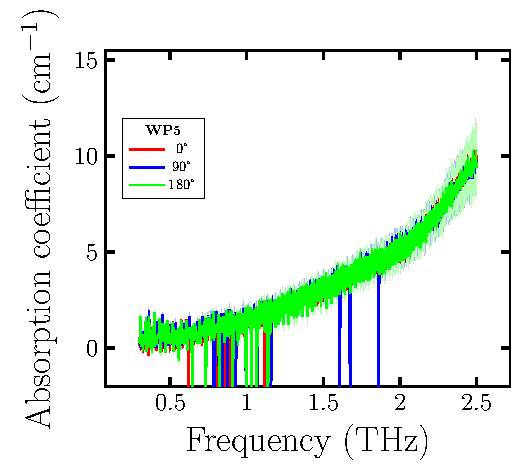
\includegraphics[width=0.45\linewidth]{images/appendix/plots/real_abs/WP5.pdf}}
\caption{Evaluated absorption coefficient for the five requested waveplates at three different rotational angles.}
\label{fig:ceramic_WPs_abs}
\end{figure}

\begin{figure}[H]
\centering
\subcaptionbox{\label{fig:ceramic_MUT1_abs}}
    {\hspace*{-2em}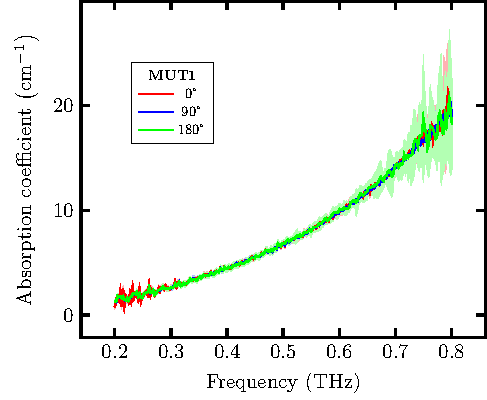
\includegraphics[width=0.45\linewidth]{images/appendix/plots/real_abs/MUT1.pdf}}
\qquad
\subcaptionbox{\label{fig:ceramic_MUT2_abs}}
    {\hspace*{-2em}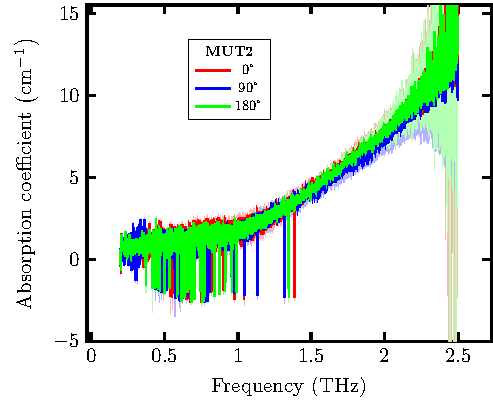
\includegraphics[width=0.45\linewidth]{images/appendix/plots/real_abs/MUT2.pdf}}
\subcaptionbox{\label{fig:ceramic_MUT3_abs}}
    {\hspace*{-2em}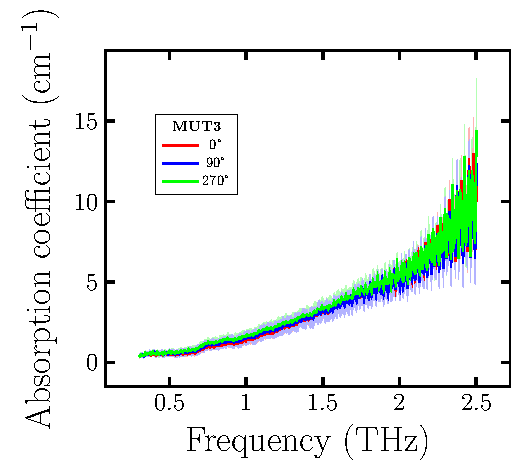
\includegraphics[width=0.45\linewidth]{images/appendix/plots/real_abs/MUT3.pdf}}
\qquad
\subcaptionbox{\label{fig:ceramic_MUT4_abs}}
    {\hspace*{-2em}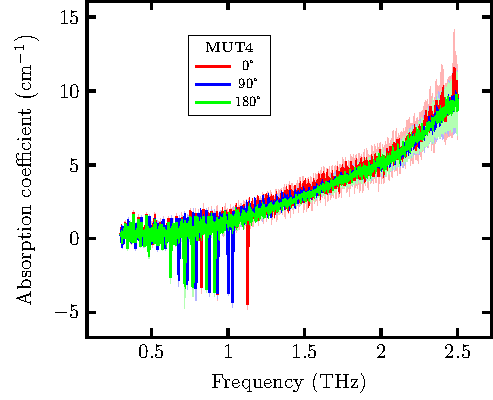
\includegraphics[width=0.45\linewidth]{images/appendix/plots/real_abs/MUT4.pdf}}
\subcaptionbox{\label{fig:ceramic_MUT5_abs}}
    {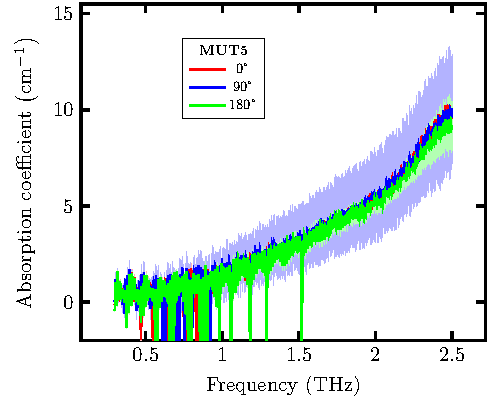
\includegraphics[width=0.45\linewidth]{images/appendix/plots/real_abs/MUT5.pdf}}
\caption{Evaluated absorption coefficient for the five additional samples at three different rotational angles.}
\label{fig:ceramic_MUTs_abs}
\end{figure}

If we compare the measured refractive index and the absorption coefficient of these \ce{Al2O3} samples to the result from the measurement published in \cite{Ornik2018} of two similar \ce{Al2O3} samples, we see that the refractive index and absorption coefficient for WP1-WP5 and MUT3-MUT5 is approximately the same. Furthermore, we see that the refractive index and absorption coefficient of MUT1 is higher than the other samples since this sample consists of \ce{ZrO2}. The material of MUT2 was either \ce{ZrO2} or \ce{Al2O3}, based on the value of the refractive index we can conclude that MUT2 consists of \ce{Al2O3}. Finally, it seems that none of the samples have a measurable birefringence except MUT2 which has a birefringence of around $0.05$. The missing birefringence could be due to a different printing process and or different printing settings.
